\section{Durchführung}
\label{sec:Durchführung}

\subsection{Elektronenstrahl im E-Feld}
\begin{figure}[H]
  \centering
  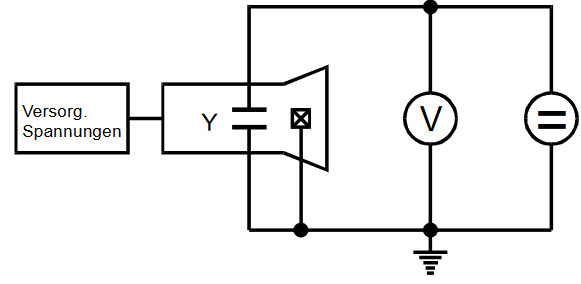
\includegraphics[height=6cm]{Elektronenstrahlroehre_Schaltung.PNG}
  \caption{Schaltung einer Kathodenstrahlröhre. \cite{sample}}
  \label{fig:Schaltung}
\end{figure}

Die Elektronenkanone der Elektronenstahlröhre wird entsprechen Abbildung \ref{fig:kathode}
an eine Heizspannug $U_G$ sowie die weiteren Fokussierungs- und Beschleunigungsspannungen angeschlossen.
Anschließend werden auch die Ablenkplatten der Röhre, wie in Abbildung \ref{fig:Schaltung} zu erkennen, mit Spannung
versorgt und geerdet.

Die Fokussierungsspannungen werden nun so eingestellt, dass ein möglichst kleiner leuchtender Punkt auf dem
Detektorschirm zu sehen ist. Bei konstanter Beschleunigungsspannung wird dann die Ablenkspannung variiert, sodass
der Punkt auf der untersten der 9 äquidistanten Linien des Schirms liegt. Die Ablenkspannung dieser Konfiguration wird
notiert. Anschließend wird der Punkt auf die nächst höhere Linie gelegt und die Spannung erneut gemessen.
Dieser Vorgang wird für alle der 9 besagten Linien und für ingesamt 5 unterschiedliche Beschleunigungsspannungen wiederholt.

\begin{figure}[H]
  \centering
  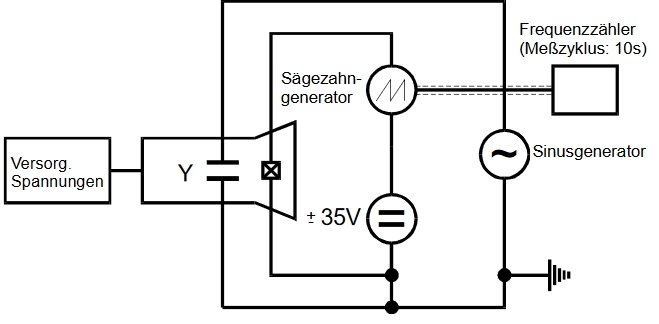
\includegraphics[height=6cm]{Oszilloskop_Schaltung.PNG}
  \caption{Prinzipielle Schaltung eines Kathodenstrahl-Oszillographen . \cite{sample}}
  \label{fig:Schaltung1}
\end{figure}

Im zweiten Teil des Versuchs werden die Ablenkplatten dann an eine Sägezahnspannung (X-Richtung)
und eine Sinusspannung (Y-Richtung) angeschlossen (Abbildung \ref{fig:Schaltung1}). Durch Variation
der Frequenz der Sägezahnspannung wird dann versucht die gewünschten Frequenzverhältnisse
der Spannungen herzustellen. Erkannt werden diese an den stehenden Bildern auf dem
Detektorschirm sowie der dann auf ihm abzählbaren Anzahl an dargestellten Halbwellen.
Die entsprechenden Frequenzen der Sägezahnspannung sowie die maximalen Strahlauslenkungen der Sinusspannung
dieser Konfigurationen werden mithilfe eines Frequenzzählers bzw. der Markierungen des Detektorschirms
gemessen und notiert.


\subsection{Elektronenstrahl im B-Feld}
Bei diesem Versuch wird eine Elektronenstrahlröhre mittig zwischen ein Helmholtz-Spulenpaar gestellt.
Sie wird dabei so ausgerichtet, dass die Flugrichtung der Elektronen senkrecht zum entstehenden Magnetfeld
verläuft und die Achse der Röhre in Richtung der Horizontalkomponente des Erdmagnetfeldes zeigt. Diese
wird mit dem Deklinatorium-Inklinatorium festgestellt. Nun wird die Kathodenstrahlröhre wieder, wie im ersten
Abschnitt des oben stehenden Versuchs bereits erklärt, an die unterschiedlichen Spannungsquellen angeschlossen (Abbildung \ref{fig:kathode}/\ref{fig:Schaltung}).
Anschließend wird durch Anpassung der Fokussierungsspannungen wieder ein möglichst kleiner leuchtender Punkt auf
dem Detektorschirm erzeugt. Dieser wird mithilfe der an die Ablenkplatten angelegten Spannungen auf die unterste
der 9 äquidistanten Linien des Schirms abgelenkt. Nun wird Strom auf die Helmholtz-Spulen gegeben. Die Stromstärke
wird so eingestellt, dass der Punkt nun auf der nächst höheren Linie liegt. Der entsprechende Wert wird notiert und
der Vorgang wird auch für die verbleibenden Linien wiederholt. Die gesamte Messung wird für die zwei gefragten
Beschleunigungsspannungen durchgeführt.

Zur Messung des Erdmagnetfeldes wird die Apparatur vorerst gleich aufgebaut. Der leuchtende Punkt wird in diesem Fall
nun aber auf einen beliebigen Punkt des Detektorschirms gelegt. Dieser wird sich gemerkt. Dann wird die
Elektronenstrahlröhre samt Spulen aus der Nord-Süd-Ausrichtung in eine Ost-West-Ausrichtung gedreht. Der Punkt hat sich
nun durch den Einfluss des Erdmagnetfeldes verschoben. Durch Anlegen eines Stroms auf die Helmholtz-Spulen und das dadurch
entstehende Magnetfeld wird dieser nun wieder in seine Ausgangposition zurückgelengt. Der benötigte Spulenstrom wird gemessen.
Anschließend wird noch mit dem Deklinatorium-Inklinatorium der Inklinationswinkel des Erdmagnetfeldes bestimmt.
